\documentclass[titlepage,a4paper]{jsarticle}
\usepackage{../sty/import}% 各種パッケージインポート
\usepackage{../sty/title_kyoudou}% タイトルページの変更

%% タイトルページの変数
% レポートタイトル
\title{Driving-saver仕様報告書}
% 提出日
\expdate{\today}
% 科目名
\subject{マルチメディア情報論}
% 分野
\class{情報経営システム工学分野}
% 学年
\grade{B3}
% 学籍番号
\mynumber{24336488}
% 記述者
\author{本間三暉}
% グループ名 % もし班があるやつならtitle_team.styを入れる
% \team{10}
% 共同実験者 % もし共同実験者が必要なやつならtitle_kyoudou.styを入れる
\coauthor{%
 \textbf{学籍番号:}24332587 & \textbf{氏名:}浅見圭介  \\
 \textbf{学籍番号:}24332990 & \textbf{氏名:}内田晴己  \\
 \textbf{学籍番号:}24333290 & \textbf{氏名:}小笠原優心 \\
 \textbf{学籍番号:}24336466 & \textbf{氏名:}松浦瑛太  \\
}
%
% 記載例:
%\coauthor{%
% 学籍番号:24567321 & 氏名:吉田 富美男 \
% 学籍番号:12345678 & 氏名:安藤 雅洋 \
% 学籍番号:13579234 & 氏名:雲居 玄道 \
%%

\begin{document}
% titleページ作成
\maketitle
\section{はじめに}
自動車安全運転センターの初心運転者の運転意識と実態に関する調査研究\cite{自動車}によると,
年間の交通事故の10人に1人以上が運転免許取得後1年未満の運転初心者である.

運転初心者は車幅感覚が身についていないことや,道路に慣れておらず正しい道の選択ができないことが原因としてあげられる.
これは,教習所の講習だけでは運転に必要な感覚が全て身につかないからではないかと考えられる.

昨今ADSD(先進運転システム)を搭載した自動車が開発・製造されている.
しかし,ADSDを搭載した車は高く,運転免許を取り立ての10代20代の経済力では手を出しにくい.

そこで,私達はADSDよりも手軽なアプローチとして運転初心者の人間が危険な道に入って事故を起こすのを防止することを目的として,
Driving-saverというシステムを提案する.
Driving-saverは車内カメラと専用マップアプリを用いて運転中に危険を通知する.
車内カメラを用いて車幅間隔を計測し,道路端とある一定以上近づいたら運転者に音で警告する.
また,そうやって集めたデータを用いて事故の起きやすい場所をマップ上に表示する.
\section{実現方法の検討}
実現方法について検討する.
\subsection{システムの全体構成}
システムの全体をユースケース図に起こしたものを図\ref{ユースケース図}に,シーケンス図に起こしたものを図\ref{シーケンス図}に,
ER図に起こしたものを図\ref{ER図}に,クラス図に起こしたものを\ref{クラス図}に示す.

\begin{figure}[H]
  \centering
  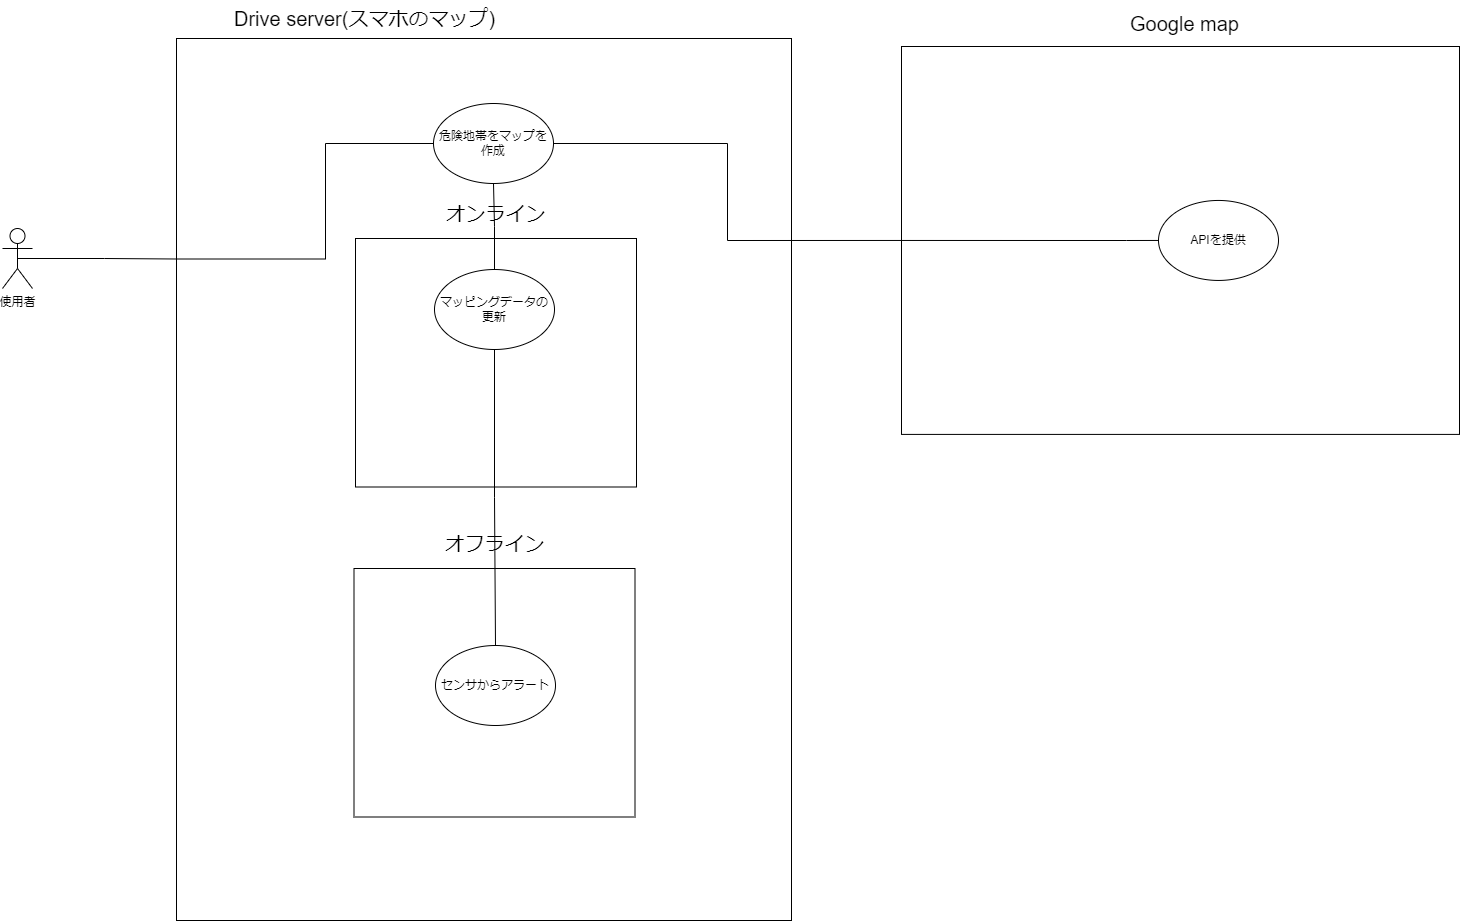
\includegraphics[width=\textwidth]{img/usecase.drawio.png}
  \caption{ユースケース図}
  \label{ユースケース図}
\end{figure}

\begin{figure}[H]
  \centering
  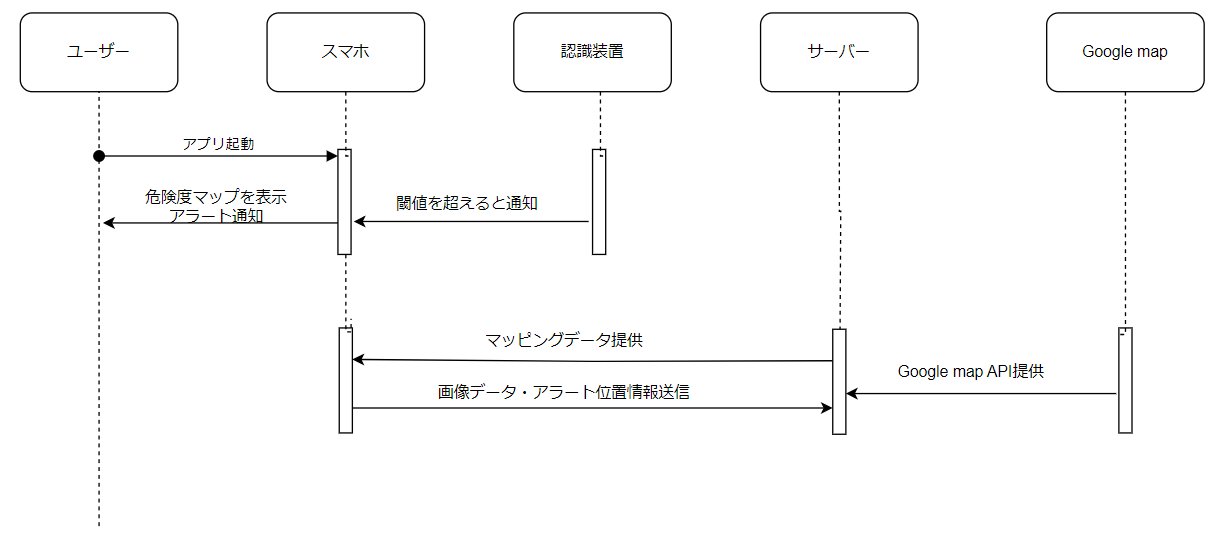
\includegraphics[width=\textwidth]{img/sea_fig.png}
  \caption{シーケンス図}
  \label{シーケンス図}
\end{figure}

\begin{figure}[H]
  \centering
  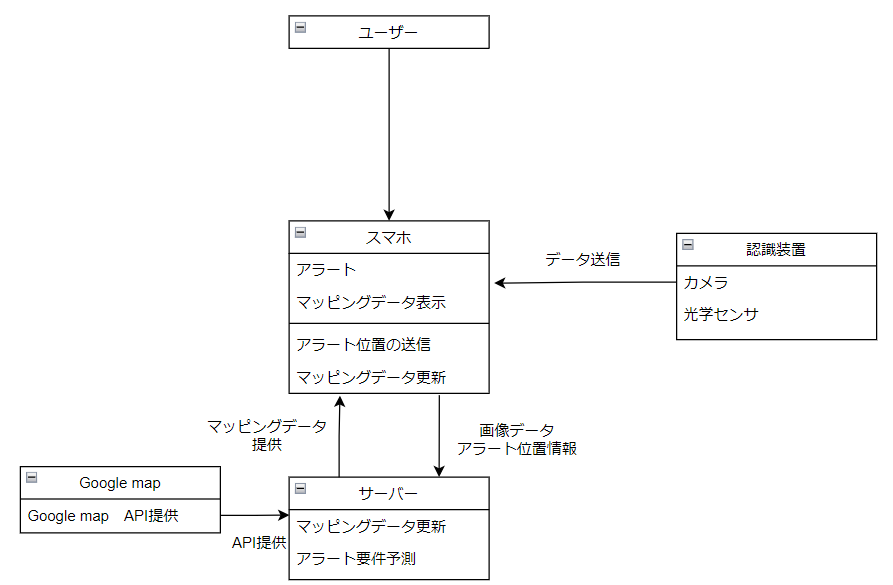
\includegraphics[width=\textwidth]{img/class_fig.png}
  \caption{クラス図}
  \label{クラス図}
\end{figure}

\begin{figure}[H]
  \centering
  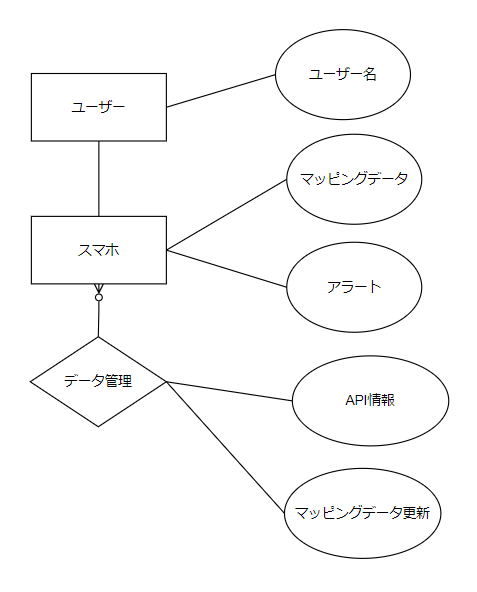
\includegraphics[width=\textwidth]{img/ER_fig.png}
  \caption{ER図}
  \label{ER図}
\end{figure}

構成要素はデバイスとソフトウェア,データベースの3つに分けられる.
\subsection{各構成要素の機能}
デバイスは
\subsection{通信方法}

\section{各要素の設計}
\subsection{利用する部品・モジュール}
\subsection{ハードウェア}
\subsection{筐体}
\subsection{ソフトウェア}

\section{今後の展望}

% 参考文献
\begin{thebibliography}{99}
  \bibitem{自動車} 「初心運転者の運転意識と実態に関する調査研究」自動車安全運転センター\\
  \url{https://www.jsdc.or.jp/Portals/0/pdf/library/research/h02_1.pdf}

\end{thebibliography}

\end{document}

